\chapter{Parte 4}
\label{cap:p4}

\section{Análise do problema}

O problema deste capítulo baseia-se no modelo apresentado no Capítulo anterior,
e pretende-se encontrar todas as soluções possíveis, a partir da duração inicial
do projeto com várias reduções, de forma a poder relacionar os custos de redução
com o custo do projeto. Desta forma, é possível fazer um balanço de quanto é que
o projeto se pode reduzir e o seu custo de redução. Ou seja, se os custos de
redução justificam a redução pretendida, qual é o máximo que se pode reduzir
e quanto custa.

\section{Modelo}

\subsection{Parâmetros}

À imagem do capítulo anterior, considerou-se a duração de cada atividade
e a suas precedências como parâmetros, bem como os custos de redução e normais
daquelas. Ao contrário das partes anteriores, usou-se os custos normais na construção do modelo. A inclusão deste custos no modelo nesta parte justifica-se pela conveniência no
cálculo dos custos totais em cada unidade que se pretende decrementar, que está
explicado sucintamente mais abaixo neste capítulo.

\subsection{Variáveis de decisão}

As variáveis de decisão são as mesmas que as descritas no Capítulo \ref{cap:p3}, secção
 \ref{p3:vardec}.\ Ou seja, pretende-se decidir qual as reduções necessárias em cada
atividade, com o menor custo total. As reduções são descritas como
anteriormente: 
$$R_i, \forall i \in \{ini, 0, 1, 3, 4,5,6,7,9,10,11,fim\}$$

De igual modo, se inclui os tempos de inicio de atividade, à semelhança do
capítulo anterior:

$$T_i, \forall i \in \{ini, 0, 1, 3, 4,5,6,7,9,10,11,fim\}$$

O significado destas últimas variáveis mantém-se (ver Capítulo \ref{cap:p3}, secção \ref{p3:vardec}).


\subsection{Função Objetivo}
 
A função objetivo sofreu uma modificação em relação ao modelo do capítulo
anterior. Nesta parte, acrescentou-se o custo normal da cada atividade à função objetivo. Assim, a função objetivo agora não representa o custo total suplementar das reduções e passa a representar o custo total do projeto, que engloba os custos normais e os custos suplementares. Continua-se a querer minimizar os custos de redução de forma ótima, apenas se
inclui o custo normal da cada atividade. Note-se que, a soma de todos os custos
normais não influência o valor das variável de decisão (ao contrário dos
custos de redução), uma vez que todas as atividades têm que ser realizadas e os seus custos normais são fixos.
Assim, o valor da função objetivo permite saber o custo total (custos normais
mais custos de redução) para redução de tempo que se pretende efetuar ao projeto.


A função objetivo, para cada atividade $i \in \{ini, 0, 1, 3,
4,5,6,7,9,10,11,fim\}$, é que figura a seguir:

\begin{displaymath} 	
	\min~z = \sum C_{\text{Normal}~i} + C_{\text{Redução}~i} \times R_{i}
\end{displaymath}

Onde:

\begin{itemize} 
	
	\item $C_{\text{Normal}~i}$ --- Custo normal da atividade $i$;

	\item $C_{\text{Redução}~i}$ --- Custo de redução da atividade $i$;
	\item $R_{i}$ --- Redução de tempo da atividade $i$ 

\end{itemize}

Concretizando os valores na função:

\begin{align*}
	\min~z&:&   &400 & +& 100~R0 & +& 1000& +& 300~R1 \\
	      & & + &300 & +& 100~R3 & +& 2000& +& 400~R4 \\
		  & & + &1000& +& 800~R5 & +&  800& +&  90~R6 \\ 
		  & & + &900 & +& 0~R7 & +&  300& +&   0~R9 \\
		  & & + &1600& +& 500~R10& +& 1400& +& 300~R11 \\
\end{align*}

\subsection{Restrições}

As restrições são iguais às da Parte III, com a exceção da restrição do
tempo final do projeto, onde, ao invés de subtrair 3 unidades de tempo ao tempo
do caminho crítico do projeto, considerou-se uma redução gradual (de 1 unidade de tempo) em cada
execução do modelo no \texttt{lp\_solve}, de forma a obter um custo total para
cada valor de redução, e por isso de cada tempo total de execução do projeto. O ponto de partida foi o tempo do projeto obtido na Parte I, de 26 unidades de tempo e a partir dai analisou-se todas as possibilidades redução de tempo até uma redução máxima de 26 unidades de tempo, que corresponde a uma duração nula do projeto. Reduções muito elevadas são impossiveis como seria de esperar, no entanto por uma questão de completudo, consideraram-se todas as possibilidades. Um
\emph{script} em \texttt{BASH} foi criado para o efeito, para executar todos os
modelos. Assim sendo, para cada execução do modelo a restrição do tempo final
fica:

$$ T_{fim} = T_{\text{caminho crítico}} - R_{\text{total desejada}}$$


\begin{itemize} 
	
	\item $T_{fim}$ --- Tempo final;
	\item $T_{\text{caminho crítico}}$ --- Tempo total do caminho crítico;
	\item $R_{\text{total desejada}}$ --- Redução total de tempo desejada no projeto,
		em cada execução do modelo no \texttt{lp\_solve}.

\end{itemize}

Assim:

\begin{align*}	
	 T_{fim}& = 26 - 0 = 26\\
	 T_{fim}& = 26 - 1 = 25\\
	 T_{fim}& = 26 - 2 = 24\\
	 T_{fim}& = 26 - 3 = 23\\
	  \dots     & \\
	 T_{fim}& = 26 - 26 = 0\\
\end{align*}

\section{\emph{Input} do \emph{script} em \emph{BASH}}

O \emph{script} para a execução de cada redução manipula o ficheiro do modelo do
\texttt{lp\_solve}, removendo a última linha onde se encontra a última
restrição, para em seguida adicionar uma nova linha com uma nova restrição
com o novo valor a reduzir. O \emph{output} apresentado corresponde à primeira
linha de cada execução do modelo. O código do \emph{script} foi o seguinte:


\begin{verbatim}
#!/bin/bash

#Nome do ficheiro passado como parâmetro de entrada
file="$1"

#Valor do tempo do caminho crítico
CAM_CRIT=26

#Redução em cada execução
REDUCAO=0
for i in $(seq $CAM_CRIT -1 0)
do
      #Formata string com última restrição com valor da redução
      var='Tfim ='$i';'
      #Elimina a última string do ficheiro
      sed -i '$ d' $file
      #Acrescenta string formatada ao final do ficheiro
      echo $var >> $file
      #Guarda 1ª linha do output de cada execução
      out=$(lp_solve $file | head -n 2) 
      #Apresenta resultado no stdin
      echo Redução de $REDUCAO : $out
      REDUCAO=$((REDUCAO + 1))
done

\end{verbatim}


\newpage

\section{Resultado}

Os valores do \emph{output} da execução do \emph{script} figuram a seguir:

\begin{verbatim}
Redução de 0 (Tfim = 26) : Value of objective function: 9700
Redução de 1 (Tfim = 25) : Value of objective function: 9790
Redução de 2 (Tfim = 24) : Value of objective function: 9880
Redução de 3 (Tfim = 23): Value of objective function: 9980
Redução de 4 (Tfim = 22): Value of objective function: 10380
Redução de 5 (Tfim = 21): Value of objective function: 10780
Redução de 6 (Tfim = 20): Value of objective function: 11180
Redução de 7 (Tfim = 19): Value of objective function: 12280
Redução de 8 (Tfim = 18): This problem is infeasible

\end{verbatim}

Como se pode observar, a partir da redução de 8 unidades de tempo,
o \texttt{lp\_solve} não consegue resolver o modelo, e portanto o output do script a partir dai foi omitido. Logo a redução máxima
possível é de 7 unidades de tempo, que representa realizar o projeto em 19 unidades de tempo, com o custo total de 12280 unidades
monetárias.

A tabela \ref{p4:tab:custos} associa as reduções possíveis ao tempo total do projeto e respetivo custo total de execução do mesmo.

\begin{table}[H]
\centering
\begin{tabular}{c c c}
\toprule
	Redução & Tempo Total & Custos Totais \\ 
\midrule
0&  26& 9700  \\ 
1&  25& 9790  \\
2&  24& 9880  \\
3&  23& 9980  \\
4&  22& 10380 \\
5&  21& 10780 \\
6&  20& 11180 \\
7&  19& 12280 \\
8&  18& $\infty$\\ 
\bottomrule
\end{tabular}
\caption{Reduções em cada execução do modelo no \texttt{lp\_solve}}
\label{p4:tab:custos}
\end{table}

 O gráfico \ref{p4:fig:grafico1} foi elaborado com base na tabela \ref{p4:tab:custos} e mostra o custo total do projeto para cada valor de redução de tempo possíveis.

\begin{figure}[H]
\centering
\resizebox{0.7\textwidth}{!}{%
\begin{tikzpicture}
	\begin{semilogyaxis}
		    [
					x tick label style={/pgf/number format/1000 sep=}, 
	grid=major,
	log ticks with fixed point,
	xlabel={Redução temporal [U.T.]},
	ylabel={Custo Total [U.M.]},
					enlargelimits=0.15, 
			ybar, bar width=7pt, 
				]

\addplot table [x=red,y=custo, color=red,] {data/res.txt};
		\end{semilogyaxis}
\end{tikzpicture}
}%
\caption{Gráfico do custo total do projeto em função das reduções de tempo}
\label{p4:fig:grafico1}
\end{figure}




O gráfico \ref{p4:fig:grafico2} mostra o custo total do projeto para cada valor de duração do projeto.

\begin{figure}[H]
	\centering
	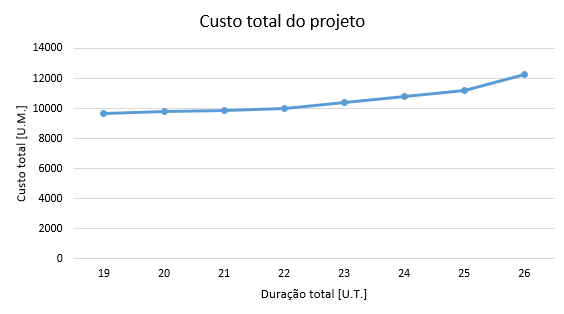
\includegraphics[scale=0.8]{./img/p4_grafico2}
	\caption{Gráfico com custo total em função da duração do projeto}
	\label{p4:fig:grafico2}
\end{figure}

Foram omitidos do gráfico reduções de tempo para as quais não existe solução do modelo.

Os resultados mostram que a duração projeto pode ser reduzida no máximo em 7 unidades  de tempo (duração total de 19 u.t) com um custo total de 12280 unidades monetárias. De igual modo, entre
a duração do projeto sem reduções e redução máxima existem mais 6 possíveis
reduções, com um custo entre 9790 U.T. e 11180 U.M. (não incluindo a máxima
redução).

Através do gráfico \ref{p4:fig:grafico2} é possível perceber os vários compromissos entre a duração total do projeto e o custo total. Nomeadamente, o gráfico sugere que para durações do projeto próximas da inicial (26 unidades de tempo), cada redução adicional não acarreta um aumento nos custos significativo. No entanto, tal já não acontece para durações do projeto mais pequenas, onde cada redução adicional tem custos suplementares elevados. Esse fator pode ser visto no gráfico pelos declives das rectas que unem os vários pontos, que vai aumentando, até ao ponto em que o problema é impossível e não é possível terminar o projeto num tempo menor.
